\documentclass{article}

\usepackage{arxiv}

\usepackage[utf8]{inputenc} % allow utf-8 input
\usepackage[T1]{fontenc}    % use 8-bit T1 fonts
\usepackage{hyperref}       % hyperlinks
\usepackage{url}            % simple URL typesetting
\usepackage{booktabs}       % professional-quality tables
\usepackage{amsfonts}       % blackboard math symbols
\usepackage{amsmath}
\usepackage{amssymb}
\usepackage{nicefrac}       % compact symbols for 1/2, etc.
\usepackage{microtype}      % microtypography
\usepackage{graphicx}
\usepackage[numbers,sort&compress]{natbib}
\usepackage{doi}
\usepackage{tikz}
\usetikzlibrary{positioning,arrows.meta,fit,backgrounds}

\title{Latent Reasoning Steps for Typed Decisions:\\Test-Time Compute for System-One Models}

\author{
	\href{https://orcid.org/0000-0001-6269-494X}
	{
\includegraphics[scale=0.06]{orcid.pdf}\hspace{1mm}Silvan Ferreira} \\
	Institute of Digital Metropolis \\
	Federal University of Rio Grande do Norte \\
	Natal, RN, Brazil \\
	\texttt{silvan.ferreira@ufrn.br}
	\And
	\href{https://orcid.org/0000-0001-5356-3550}
	{
\includegraphics[scale=0.06]{orcid.pdf}\hspace{1mm}Thiago Medeiros} \\
	Campus Natal-Zona Leste \\
	Federal Institute of Rio Grande do Norte \\
	Natal, RN, Brazil \\
	\texttt{thiago.medeiros@ifrn.edu.br}
	\And
	\href{https://orcid.org/0000-0002-0116-6489}
	{
\includegraphics[scale=0.06]{orcid.pdf}\hspace{1mm}Ivanovitch Silva} \\
	Department of Computer Engineering and Automation \\
	Federal University of Rio Grande do Norte \\
	Natal, RN, Brazil \\
	\texttt{ivanovitch.silva@ufrn.br}
}

\renewcommand{\shorttitle}{Latent Reasoning Steps for Typed Decisions}

\hypersetup{
pdftitle={Latent Reasoning Steps for Typed Decisions: Test-Time Compute for System-One Models},
pdfsubject={Machine Learning, Reasoning, Test-Time Compute},
pdfauthor={Silvan Ferreira, Thiago Medeiros, Ivanovitch Silva},
pdfkeywords={latent reasoning, test-time compute, recurrent depth, structured output, calibration, length generalization},
}

\date{}

\newcommand{\zr}{\textsc{z-reason}}

\begin{document}
\maketitle

\begin{abstract}
Recently released System-One models such as Jev answer typed questions about a state with calibrated probabilities over a predefined set of answers, instead of generating text. Their output is type safe by construction and a single fast forward pass answers every question, but the same amount of computation is spent on easy and hard questions alike, so these models cannot benefit from test-time compute. We study a simple way to add it. We present \zr{}, a small model that keeps the same request and response interface, namely a state, a set of independent \emph{choice}, \emph{score} and \emph{noul} questions, and probabilities over the answers that each request supplies. Between encoding and read-out, the model iterates a weight-tied block over a latent state $z$ for a number of steps chosen by the user, much as a diffusion sampler runs a chosen number of denoising steps. The recurrence operates on one vector per fact of the state rather than on characters, and the number of steps is sampled at random during training. On a synthetic variable tracking task whose difficulty is the length of a dependency chain, a model with 4.1M parameters trained on chains of at most 8 hops answers chains of up to 16 hops with at least 99\% accuracy when given 8 or more steps, in each of three seeds. At three to four times the training depth the extrapolation becomes partial and depends on the seed, with accuracy between 63\% and 100\% at 32 steps. A transformer without weight tying and with 15.1M parameters, trained in the same way, falls close to a root guessing baseline as soon as the depth exceeds its training range. The number of steps needed grows sublinearly with depth. When the same architecture is trained with a fixed number of steps it extrapolates only at particular step counts, whereas after random step training, steps added beyond the point of near perfect accuracy cost at most about one point. Calibration error decreases as steps increase, and a simple convergence rule for halting spends more steps on harder questions without losing accuracy. We also report the design choices without which the model did not learn. All results come from a single synthetic task, so they show the mechanism at work in a controlled setting and do not yet speak to decisions over natural language.
\end{abstract}

\keywords{Latent reasoning \and Test-time compute \and Recurrent depth \and Structured output \and Calibration \and Length generalization}

\section{Introduction}
\label{sec:introduction}

Most of the reasoning done by language models today happens in text. The model writes a chain of thought and conditions its answer on it \cite{wei2022chain}, and writing more of it tends to buy accuracy \cite{snell2024scaling}. A large class of applications, however, has no use for the text itself. Routing a support ticket, grading an answer against a rubric or checking whether a record satisfies a condition all ask for a decision of a known type that downstream code will consume. TypeSafe's Jev \cite{typesafe2026jev, typesafe2026docs} turns this into the entire interface. A request contains a state and a set of independent questions of three kinds. A \emph{choice} question selects one of up to 255 options, a \emph{score} question places the state on between 2 and 10 ordered levels, and a \emph{noul} question returns the probability that a proposition holds. The response gives the typed value, a probability for every option and a confidence derived from the shape of that distribution. Since the model only assigns probabilities to answers supplied by the request, it cannot return an answer of the wrong type or one outside the schema, and a single pass answers all questions in parallel. The price, pointed out by early commentators, is that such a model has no way to spend more computation on a harder question.

This paper asks whether test-time compute can be brought back without giving up the typed interface. Our model, \zr{}, keeps Jev's request and response format and inserts a recurrent computation in latent space between the encoding of the input and the read-out of the answer. A weight-tied block is applied to a latent state $z$ a number of times set by the user through a \texttt{steps} parameter. The user sees something close to the number of denoising steps of a diffusion sampler \cite{ho2020ddpm}, and our question is whether the analogy holds, that is, whether more steps make the model more capable and whether harder inputs need more of them.

There are good reasons to expect it might. Recurrent networks trained on easy instances of an algorithmic problem can solve harder instances when they are iterated for longer at test time \cite{schwarzschild2021learn, bansal2022endtoend}. Recurrent-depth language models scale their reasoning by iterating a block in latent space \cite{geiping2025scaling}, and small recursive models obtain strong results on puzzles by repeatedly refining a latent state together with an answer \cite{wang2025hrm, jolicoeur2025trm}. The recurrence we use is therefore not new. What we contribute is its placement behind a typed, calibrated and schema-safe decision interface, the exposure of the number of steps as a parameter of each request, and a careful measurement of the result on a task whose difficulty is controlled and whose shortcuts are measured.

Section~\ref{sec:method} describes \zr{}, which reproduces Jev's public request and response schema, encodes answer options from their text so that each request defines its own answer set, and reasons over one latent vector per fact of the state. Section~\ref{sec:task} introduces a variable tracking task with an explicit depth parameter and a measured shortcut baseline. In Section~\ref{sec:results} we show that accuracy on a question of depth $d$ rises from the level of the shortcut to at least 99\% once the number of steps passes a threshold that depends on $d$, that the model extrapolates reliably to twice its training depth and partially to four times that depth, and that a transformer without weight tying and with 3.7 times as many parameters collapses outside its training range. The same section measures how steps interact with training and calibration. The number of steps needed grows sublinearly with depth, random step training makes additional steps almost free of regressions while fixed step training does not, calibration error falls as steps increase, and a convergence rule for halting gives more steps to deeper questions. Section~\ref{sec:lessons} reports the design choices without which the model failed to learn multi-hop lookup at all, since anyone reproducing the approach at a small scale is likely to meet the same obstacles.

Table~\ref{tab:claims} summarizes which claims the experiments support and which remain open. The main limitation is one of scope. Every result comes from a single synthetic task with a clean, character-level input format, and we do not show that the approach carries over to states written in natural language, which is where a model like Jev operates.

\begin{table}[t]
\centering
\small
\caption{Claims of this paper and their status. Supported always refers to the synthetic task of Section~\ref{sec:task}.}
\label{tab:claims}
\begin{tabular}{@{}p{5.4cm}p{2.3cm}p{6.0cm}@{}}
\toprule
Claim & Status & Evidence or open question \\
\midrule
More test-time steps solve harder questions & supported & Table~\ref{tab:steps}, Figures~\ref{fig:trace} and~\ref{fig:heatmap}, three seeds \\
Extrapolation beyond the training depth by adding steps & supported up to $2\times$, partial at $3$ to $4\times$ & at least 99\% up to depth 16 in all seeds with 8 steps; between 63\% and 100\% at depths 28 to 32, depending on the seed and not monotone in steps, Table~\ref{tab:deep} \\
Steps needed grow sublinearly with depth & supported as a behavior & Figure~\ref{fig:needed}; the attention analysis does not show a clean pointer doubling mechanism \\
Random step training is needed for nearly monotone gains & supported & the fixed step baseline oscillates, Figure~\ref{fig:baselines}, in line with \cite{bansal2022endtoend, yang2026stars} \\
Calibration improves with steps & weakly supported & ECE falls with steps, Table~\ref{tab:calibration}, but saturated accuracy limits the test \\
Halting by convergence allocates compute by difficulty & supported & Table~\ref{tab:auto} \\
Transfer to natural-language states & not tested & requires a pretrained encoder and real decision data \\
A calibration objective equivalent to Jev's RLCD & not tested & we use proper scoring rules only \\
\bottomrule
\end{tabular}
\end{table}

\section{Background and Related Work}
\label{sec:related}

This work sits between two lines of research that have developed mostly apart. One builds models that return typed and calibrated decisions instead of text, and the other gives models extra computation at inference time, either by generating reasoning tokens or by iterating in a latent space. We first describe the typed decision models that motivate the interface, then the work on latent reasoning and weight sharing across depth from which the architecture is taken, and finally the studies of extrapolation from easy to hard instances that are closest to our experiments.

\paragraph{Typed decision models.} According to its developers, Jev \cite{typesafe2026jev} is a transformer trained on synthetic data with a method called Reinforcement Learning for Calibrated Decisions, or RLCD, which optimizes the stated probabilities against outcomes rather than against human preference. Its architecture, weights and training details are not public, so we rely only on its public interface \cite{typesafe2026docs}, which we reproduce, and on its stated limitation of not using test-time compute. The \emph{score} primitive returns the mean of the level indices weighted by their probabilities, and the confidence reflects how concentrated the answer distribution is. We adopt both conventions. By calibration we mean that stated probabilities match empirical frequencies \cite{guo2017calibration}. Calibration is the optimum of any strictly proper scoring rule \cite{gneiting2007scoring}, and this is how we pursue it.

\paragraph{Test-time compute and latent reasoning.} Chain-of-thought prompting \cite{wei2022chain} and its scaling at test time \cite{snell2024scaling} spend extra computation by generating tokens. A second line of work spends it in continuous space. Coconut feeds hidden states back as input instead of decoding them \cite{hao2024coconut}, and Huginn iterates a recurrent block over a latent state for a number of steps sampled at random during training, which lets it scale reasoning at inference without producing tokens \cite{geiping2025scaling}. Our training recipe follows Huginn, with step counts drawn from a heavy-tailed distribution, truncated backpropagation and a noisy initial state. Joint-embedding predictive architectures \cite{lecun2022path, assran2023ijepa} and concept-level language models \cite{barrault2024lcm} likewise move prediction from tokens to a learned representation space, and from the latter we take the idea of computing over one vector per sentence or fact.

\paragraph{Weight sharing across depth.} Universal Transformers apply one block repeatedly and learn when to halt \cite{dehghani2019universal}, building on adaptive computation time \cite{graves2016adaptive} and PonderNet \cite{banino2021pondernet}. Looped transformers can emulate programs \cite{giannou2023looped}, learn learning algorithms \cite{yang2024looped}, generalize to longer inputs when the number of loops grows with the input \cite{fan2024looped} and simulate multi-step reasoning with a depth proportional to the number of reasoning steps \cite{saunshi2025reasoning}. Deep equilibrium models solve for a fixed point of a single layer with the input injected at every iteration \cite{bai2019deq}, and we use the same additive injection. Transformers can compose $k$ lookups in depth logarithmic in $k$ \cite{sanford2024logdepth}, and our curve of required steps resembles this behavior.

\paragraph{Extrapolation from easy to hard instances.} The closest precedent for our main result is the work on deep thinking networks. Recurrent networks trained on small mazes, prefix sums or chess puzzles solve larger instances when run for more iterations \cite{schwarzschild2021learn}, and input injection combined with a progressive loss prevents overthinking, the loss of accuracy when a network iterates for too long \cite{bansal2022endtoend}. More recent work on recursive reasoners adds noise to trajectories and selects among them with a learned confidence head \cite{sghaier2026ptrm}, feeds read-out probabilities back into the recurrence \cite{kamiya2026rofb}, stabilizes looped language models with random loop sampling and spectral regularization so that more loops do not hurt accuracy \cite{yang2026stars}, iterates output embeddings to a fixed point \cite{feinashley2026attractor} and uses recurrent depth to produce outputs that are not tokens, such as robot actions \cite{tur2026rdvla}. Our comparison between fixed and random step training reproduces the overthinking phenomenon in a new setting. We did not find earlier work that puts a recurrent latent reasoner behind a typed and calibrated answer set defined per request and evaluates calibration as a function of the number of steps, although our search was not exhaustive.

\paragraph{Controlled reasoning tasks.} Our task is a variant of the variable tracking task of RULER \cite{hsieh2024ruler}. It makes chain length an explicit difficulty parameter and keeps the program size fixed so that the length of the input does not reveal the difficulty.

\section{Method}
\label{sec:method}

\zr{} has three parts. The interface fixes what a request contains and what the model returns, and it follows Jev's public schema so that the only visible addition is the number of steps. The architecture encodes the state, the question and the answer options into vectors and then refines a latent state over those vectors for the requested number of steps before reading out the answer. The training procedure is what allows a single set of weights to answer after any number of steps. We describe each part in turn and close the section with the rule used when the model decides by itself when to stop.

\subsection{Interface}

A request consists of a state $s$ and a set of questions $\{q_1, \dots, q_Q\}$. Each question has a type $\tau \in \{\text{choice}, \text{score}, \text{noul}\}$ and free-text instructions, and \emph{choice} and \emph{score} questions also carry a list of $K$ answer options written as text, which corresponds to the \texttt{criteria} field of Jev's API. For every question the model returns a probability vector $p \in \Delta^{K-1}$, or a single probability for a \emph{noul} question, together with the quantities defined by Jev's schema,
\begin{equation}
\text{choice} = \arg\max_k p_k, \qquad \text{score} = \sum_{k=0}^{K-1} k\, p_k, \qquad \text{confidence} = 1 - \frac{H(p)}{\log K}.
\label{eq:derived}
\end{equation}
The request also carries the number of latent steps $T$, which is either an integer or \texttt{"auto"}. Questions are answered independently, and no question can attend to another.

The network never emits tokens, and this is what makes the output type safe by construction. For \emph{choice} and \emph{score} questions it produces one logit per option supplied in the request, the unused positions of the padded option tensor are set to $-\infty$ before the softmax, and deterministic code then assembles the JSON response from these tensors. The model can pick a wrong option, but it cannot return an option that is not in the request, a value of the wrong type or a malformed response. This is the same guarantee behind Jev's claim of not hallucinating, which concerns the schema and not the correctness of the decision.

\subsection{Architecture}

\begin{figure}[t]
\centering
\resizebox{\textwidth}{!}{%
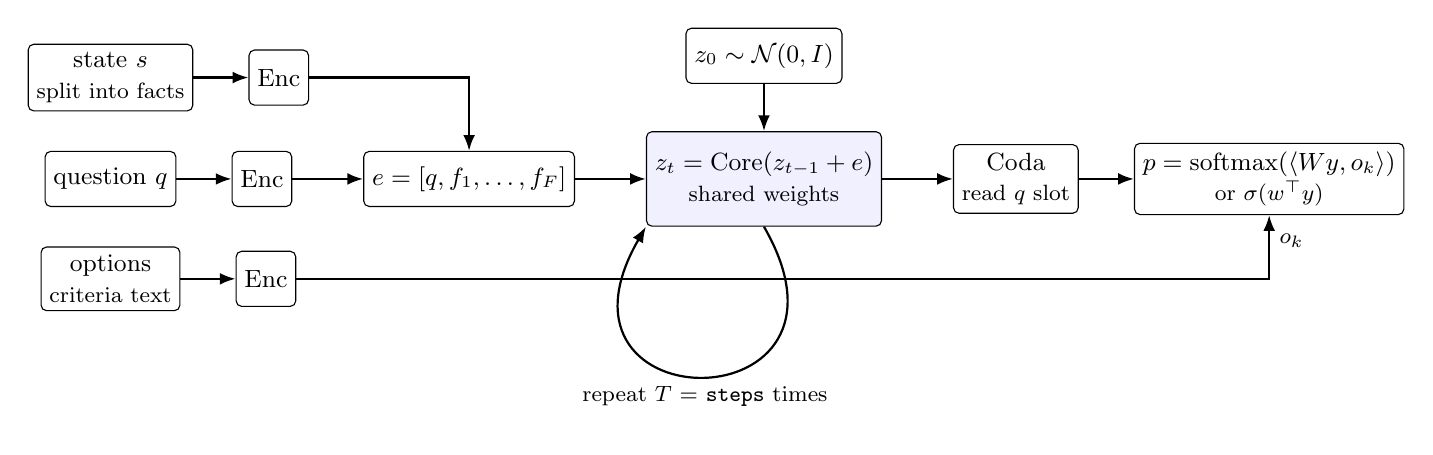
\begin{tikzpicture}[
  font=\small,
  box/.style={draw, rounded corners=2pt, minimum height=7mm, inner sep=3pt, align=center},
  arr/.style={-{Latex[length=2mm]}, thick},
  node distance=5mm and 7mm]
\node[box] (state) {state $s$\\\footnotesize split into facts};
\node[box, below=of state] (question) {question $q$};
\node[box, below=of question] (options) {options\\\footnotesize criteria text};
\node[box, right=of state] (encf) {$\mathrm{Enc}$};
\node[box, right=of question] (encq) {$\mathrm{Enc}$};
\node[box, right=of options] (enco) {$\mathrm{Enc}$};
\node[box, right=9mm of encq, minimum width=18mm] (e) {$e = [q, f_1, \dots, f_F]$};
\node[box, right=9mm of e, fill=blue!6, minimum width=26mm, minimum height=12mm] (core) {$z_t = \mathrm{Core}(z_{t-1} + e)$\\\footnotesize shared weights};
\node[box, above=6mm of core] (noise) {$z_0 \sim \mathcal{N}(0, I)$};
\node[box, right=9mm of core] (coda) {$\mathrm{Coda}$\\\footnotesize read $q$ slot};
\node[box, right=of coda] (heads) {$p = \mathrm{softmax}(\langle W y, o_k \rangle)$\\\footnotesize or $\sigma(w^\top y)$};
\draw[arr] (state) -- (encf);
\draw[arr] (question) -- (encq);
\draw[arr] (options) -- (enco);
\draw[arr] (encf) -| (e);
\draw[arr] (encq) -- (e);
\draw[arr] (e) -- (core);
\draw[arr] (noise) -- (core);
\draw[arr] (core.south) to[out=-60, in=-120, looseness=5] node[below, font=\footnotesize] {repeat $T$ = \texttt{steps} times} (core.south west);
\draw[arr] (core) -- (coda);
\draw[arr] (coda) -- (heads);
\draw[arr] (enco) -| node[pos=0.8, right, font=\footnotesize] {$o_k$} (heads);
\end{tikzpicture}}
\caption{Overview of \zr{}. A shared character-level encoder turns each fact of the state, each question and each answer option into one vector. For every question, a weight-tied core processes the set $[q, f_1, \dots, f_F]$ $T$ times, starting from a noisy latent state and injecting the encoded set again at every step. The answer distribution is read from the question slot by comparing it with the option embeddings.}
\label{fig:architecture}
\end{figure}

Figure~\ref{fig:architecture} gives an overview of the model. The state is split into facts at semicolons and line breaks. Every fact, the instructions of every question and every answer option become a short character sequence that starts with a special token, and a shared encoder of $n_{\text{enc}} = 2$ pre-norm transformer blocks with learned positional embeddings maps each sequence to a single vector through mean pooling over its tokens followed by RMS normalization. For a question $q$ we form the set $e = [\,q, f_1, \dots, f_F\,] + \kappa$, where $\kappa$ adds a learned embedding that marks the question slot. Facts receive no positional encoding, so the state is treated as a set.

The latent state starts from $z_0 \sim \mathcal{N}(0, \sigma^2 I)$ with $\sigma = 1$ and is updated as
\begin{equation}
z_t = \mathrm{RMSNorm}\big(\mathrm{Core}(z_{t-1} + e)\big), \qquad t = 1, \dots, T,
\label{eq:recurrence}
\end{equation}
where $\mathrm{Core}$ consists of $n_{\text{core}} = 2$ transformer blocks with full attention over the set, shared across all steps. Adding $e$ at every step gives the input an identity path into each iteration, as in deep equilibrium models \cite{bai2019deq}. Since each question has its own set, questions are evaluated independently and their order has no effect.

After the last step, one coda block is applied to $z_T$ and the question slot is read as the answer vector $y$. For \emph{choice} and \emph{score} questions the logits are $\ell_k = \langle W_q y,\, W_o o_k\rangle / \sqrt{d}$, where $o_k$ is the encoded text of option $k$, and for \emph{noul} questions the output is $p = \sigma(w^\top y + b)$. The main model has width $d = 256$, 8 attention heads and 4.10M parameters.

\subsection{Training}

The loss is cross-entropy for \emph{choice} and \emph{score} questions and binary cross-entropy for \emph{noul} questions, with an extra squared earth mover's distance between the predicted and target cumulative distributions for \emph{score} questions so that ordinal distance is penalized. Cross-entropy and binary cross-entropy are strictly proper scoring rules \cite{gneiting2007scoring}, which means their optimum is the calibrated distribution. We make no attempt to reproduce RLCD.

Following \cite{geiping2025scaling}, every batch runs $T = 1 + \mathrm{Poisson}(\lambda)$ steps, with $\lambda$ drawn from a log-normal distribution of mean 11 and $T$ capped at 32. Gradients flow only through the last 8 steps, so memory does not grow with $T$. The same weights therefore have to produce an answer after any number of steps, and this is what allows \texttt{steps} to be chosen at inference time.

An adaptive curriculum controls a difficulty level $\ell \in [0, 1]$ that sets both the size of the program, from 2 to 40 variables, and the maximum chain depth, from 1 to 8. The level rises by $0.1$ whenever an exponential moving average of the training accuracy on \emph{choice} questions exceeds $0.8$, at most once every 200 iterations. Every run reaches the full training distribution after about 2{,}500 of its 12{,}000 iterations.

We optimize with AdamW \cite{loshchilov2019adamw}, a learning rate of $3\times10^{-4}$, $\beta = (0.9, 0.95)$ and weight decay $0.05$ on matrices, with 500 warm-up iterations followed by cosine decay, gradient clipping at 1, batches of 128 programs with 4 questions each and bfloat16 autocast. A run takes about 48 minutes on a single RTX~3060 with 12~GB of memory.

\subsection{Inference and halting}

When \texttt{steps} is an integer, the model runs exactly that many iterations. When it is \texttt{"auto"}, the model keeps iterating until no answer probability of any question changes by more than $10^{-3}$ between two consecutive steps, with a maximum of 128 steps. This is a heuristic rule, simpler than a learned halting head \cite{graves2016adaptive, banino2021pondernet}.

\section{Task: Variable Tracking with a Depth Parameter}
\label{sec:task}

A state is a shuffled program of assignments over 52 single-character variable names, the lowercase and uppercase letters of the alphabet, as in
\begin{center}
\texttt{q=4;m=q;Z=m;c=7;k=c;w=2;T=w;A=T;B=A;C=B;D=C;E=D}.
\end{center}
A root assigns a digit and every other variable copies another variable, so the program is a set of chains. The value of a variable at depth $d$ can only be found by following $d$ assignments back to its root. Each program contains one chain of depth exactly $d$ and further chains of random length no greater than $d$, and it always holds between 24 and 40 variables. Because this range is the same in training and testing, the length of the input does not reveal the difficulty. Chains never branch.

Every state comes with four independent questions whose types are drawn uniformly. A \emph{choice} question \texttt{val x} asks for the value of \texttt{x} among 10 options, a \emph{score} question \texttt{lvl x} asks in which of five ordered buckets \texttt{0-1}, \dots, \texttt{8-9} that value falls, and a \emph{noul} question \texttt{dep x y} asks whether \texttt{x} depends on \texttt{y}, with positives and negatives equally likely. One question concerns the deepest variable of the main chain and the other three concern random variables. The difficulty of a question is the depth of the variable it asks about.

A model that does not follow the chain can still guess uniformly among the digits assigned at the roots, and we report the expected accuracy of this root guessing baseline at every depth. It goes from about 20\% at shallow depths to between 35\% and 40\% at depth 16 and to 50\% at depth 32, because a deeper main chain leaves fewer variables for the other chains and therefore fewer roots. An earlier version of the task, in which the variables formed a random forest, allowed this shortcut to reach a high accuracy on deep questions. We noticed the problem because accuracy increased with depth, and we replaced that version with the design described here.

Training uses depths 1 to 8. The main test set has 250 programs per depth for depths 1 to 16, and a second test set has 250 programs per depth for depths 16 to 32. Since only one question per program targets the deepest variable, the number of test questions per depth goes from about 2{,}500 at depth 1 to about 270 at depth 16, with again about 270 at depth 32, and roughly a third of them are \emph{choice} questions. Test programs come from random streams independent of those used in training, and with more than $10^{30}$ possible programs an exact overlap is negligible. Beyond depth 32 the limit of 52 names forces most variables into the main chain, the number of roots approaches one and the root guessing baseline approaches 100\%, so we do not report results in that range.

\section{Experiments}
\label{sec:results}

We train the main model with three seeds and compare it with two baselines trained on the same data with the same curriculum, optimizer and number of iterations. The \emph{fixed-8} baseline has the same architecture but is always trained with $T = 8$. The \emph{untied} baseline replaces the weight-tied core with eight distinct two-block cores applied once each, which gives a standard transformer with the depth and compute of eight steps and 15.1M parameters. Unless stated otherwise we report accuracy on \emph{choice} questions, which have a chance level of 10\% and require following the whole chain. Figures show the mean over seeds, with the standard deviation shaded where it is visible.

\subsection{More steps solve harder questions}

\begin{table}[t]
\centering
\small
\caption{Accuracy of \zr{} on \emph{choice} questions in percent, by question depth and number of test-time steps, as mean $\pm$ standard deviation over three seeds. The last column is the root guessing baseline. Training depth is at most 8 and $^\dagger$ marks depths never seen in training.}
\label{tab:steps}
\resizebox{\textwidth}{!}{\begin{tabular}{lccccccccc}
\toprule
& \multicolumn{8}{c}{test-time steps} & root \\
\cmidrule(lr){2-9}
depth & 1 & 2 & 3 & 4 & 6 & 8 & 16 & 128 & guess \\
\midrule
1 to 4 & 51.3\,$\pm$\,1.5 & 89.8\,$\pm$\,4.0 & 100.0\,$\pm$\,0.1 & 100.0\,$\pm$\,0.0 & 100.0\,$\pm$\,0.0 & 100.0\,$\pm$\,0.0 & 100.0\,$\pm$\,0.0 & 100.0\,$\pm$\,0.0 & 23.4 \\
5 to 8 & 35.5\,$\pm$\,1.6 & 44.7\,$\pm$\,0.8 & 72.8\,$\pm$\,3.9 & 96.4\,$\pm$\,2.0 & 100.0\,$\pm$\,0.0 & 100.0\,$\pm$\,0.0 & 100.0\,$\pm$\,0.0 & 100.0\,$\pm$\,0.0 & 26.8 \\
9 to 12$^\dagger$ & 39.4\,$\pm$\,1.2 & 46.1\,$\pm$\,1.6 & 56.5\,$\pm$\,1.2 & 69.8\,$\pm$\,2.4 & 99.1\,$\pm$\,0.7 & 100.0\,$\pm$\,0.0 & 100.0\,$\pm$\,0.0 & 100.0\,$\pm$\,0.0 & 29.7 \\
13 to 16$^\dagger$ & 42.9\,$\pm$\,1.5 & 51.8\,$\pm$\,0.9 & 64.0\,$\pm$\,2.2 & 72.9\,$\pm$\,1.3 & 90.0\,$\pm$\,1.7 & 99.3\,$\pm$\,0.5 & 100.0\,$\pm$\,0.0 & 99.9\,$\pm$\,0.1 & 31.6 \\
\bottomrule
\end{tabular}
}
\end{table}

\begin{figure}[t]
\centering
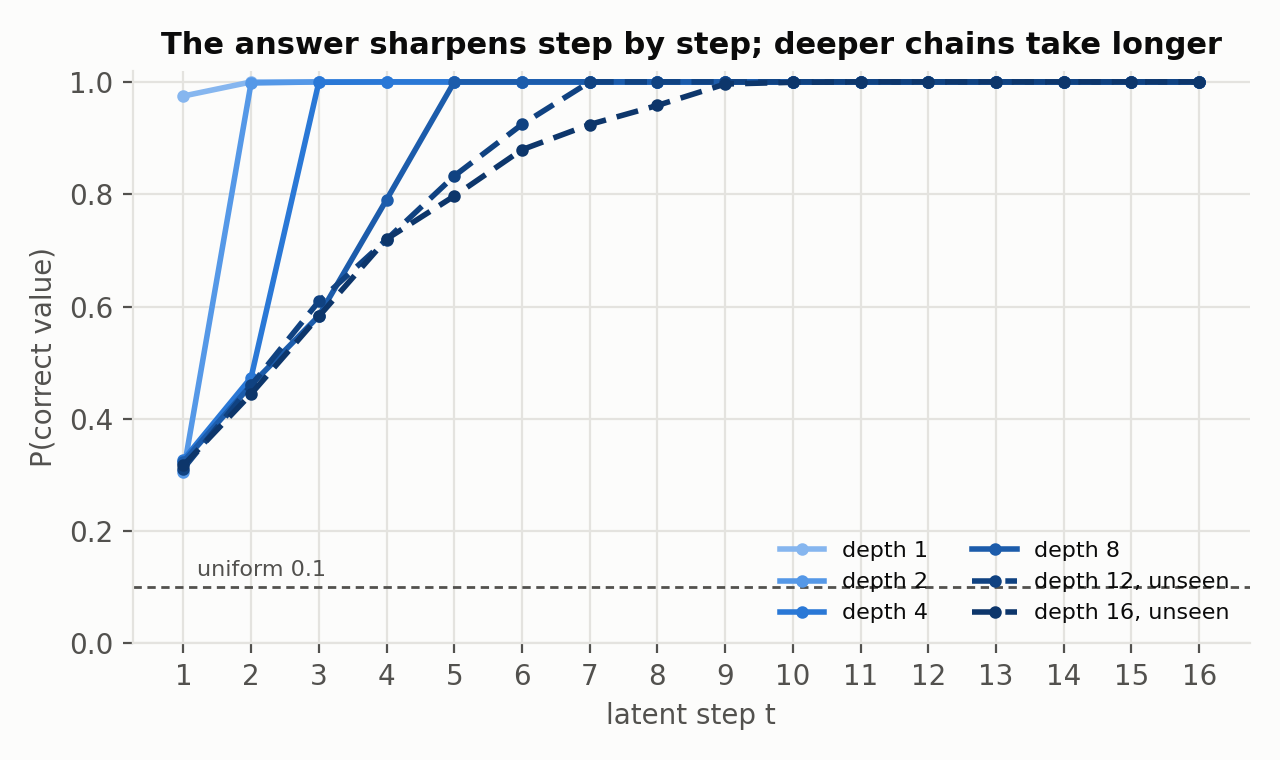
\includegraphics[width=0.62\textwidth]{figures/fig0_trace.png}
\caption{Probability assigned to the correct value after each latent step, for \emph{choice} questions about variables at different depths of the same program, averaged over 200 programs with the model of seed 0. The answer sharpens step by step, and questions about deeper variables take longer. Depths 12 and 16 were never seen in training.}
\label{fig:trace}
\end{figure}

\begin{figure}[t]
\centering
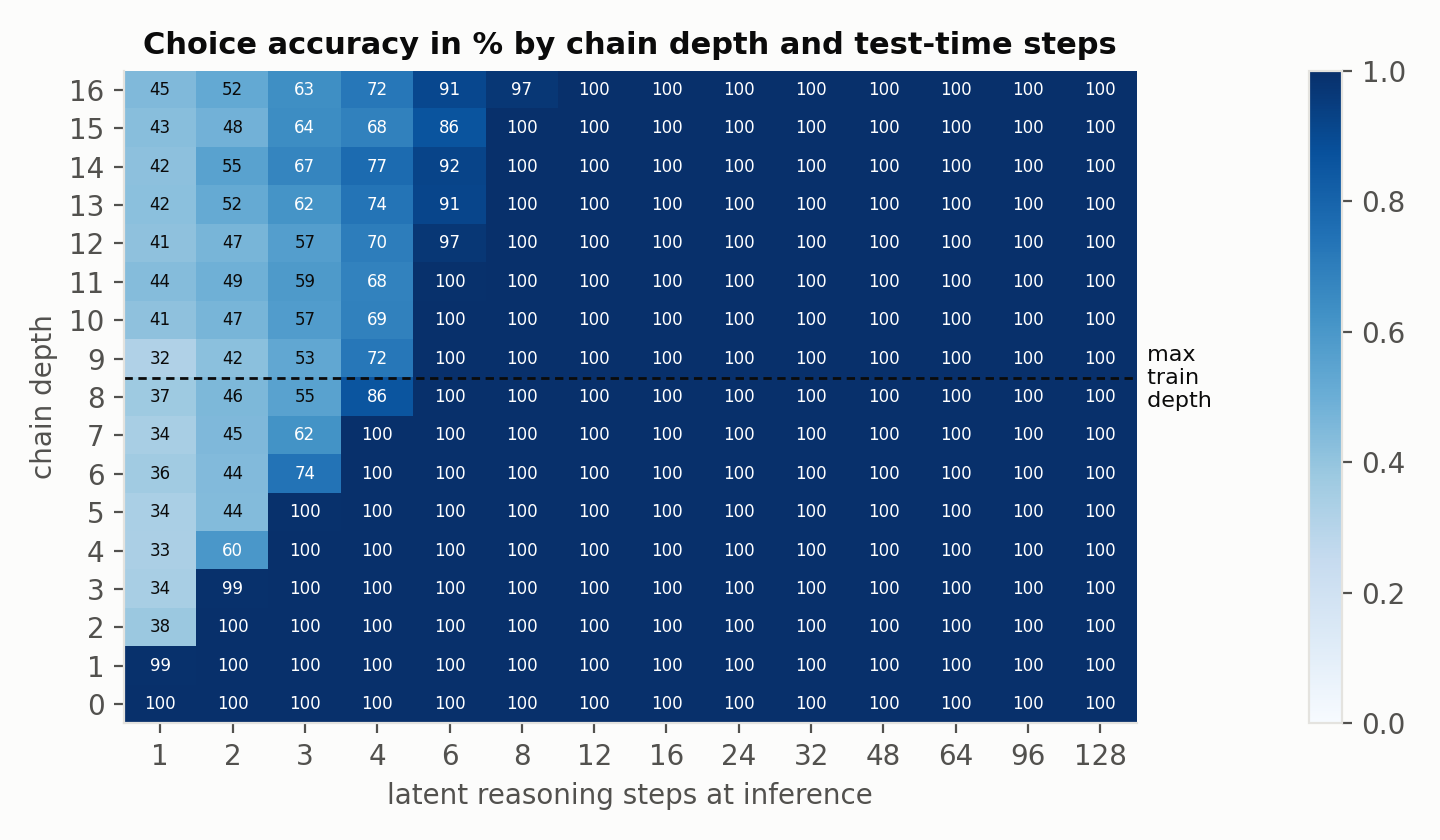
\includegraphics[width=0.8\textwidth]{figures/fig2_heatmap.png}
\caption{Accuracy on \emph{choice} questions in percent by question depth and number of test-time steps, averaged over three seeds. The dashed line marks the maximum training depth.}
\label{fig:heatmap}
\end{figure}

Table~\ref{tab:steps} and Figure~\ref{fig:heatmap} contain the central result. With one or two steps, accuracy on questions deeper than one or two hops stays close to the root guessing baseline, and each additional step widens the range of depths that the model answers almost perfectly. With four steps every seed answers depths up to 7 with at least 99\% accuracy, and with eight steps depths up to 15 are answered perfectly and depth 16 with at least 94\%. Depths never seen in training follow the same pattern, so it is the extra steps, and not extra training data, that extend the range of solved depths. Figure~\ref{fig:trace} shows the effect inside individual programs. For a fixed program, the probability of the correct value of a variable at depth $d$ grows over the first steps and saturates later when $d$ is larger, which is the behavior one would want from a decision model that can be stopped at any time.

\subsection{Steps needed grow sublinearly with depth}

\begin{figure}[t]
\centering
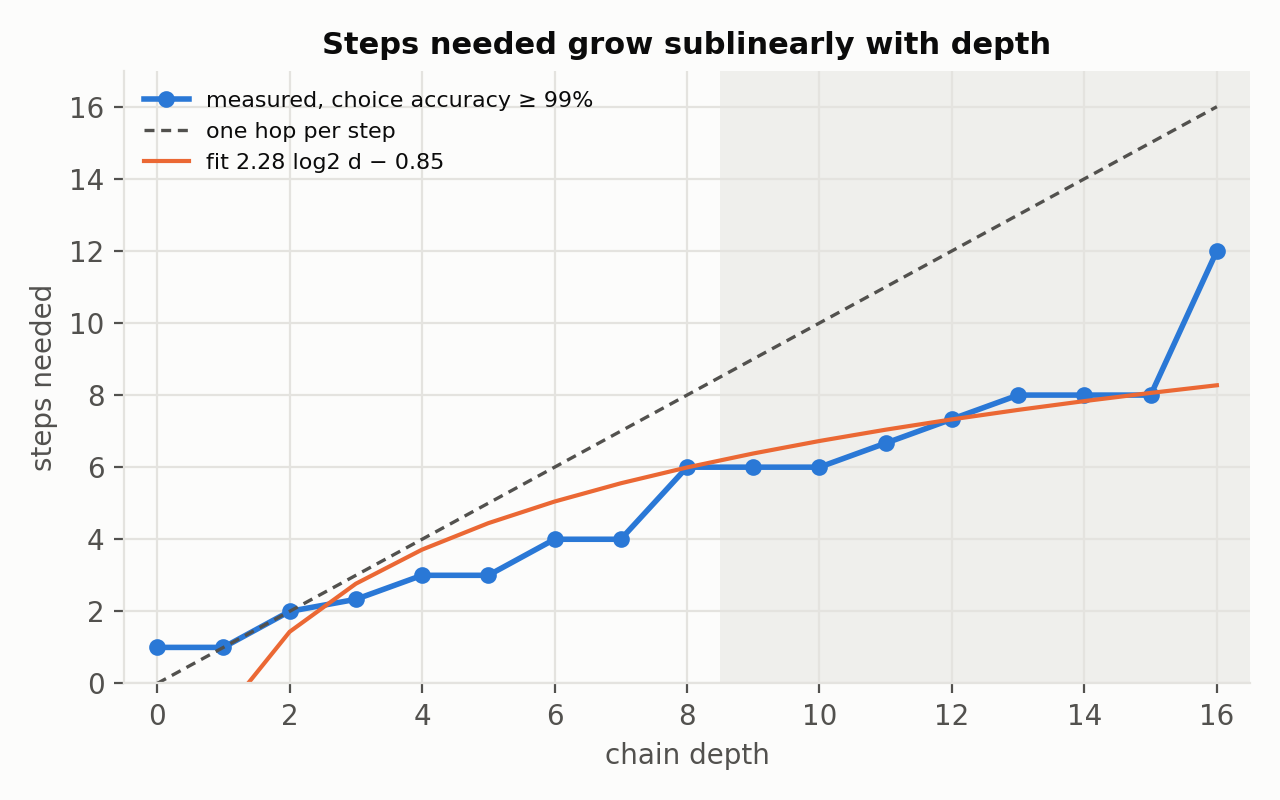
\includegraphics[width=0.62\textwidth]{figures/fig6_steps_needed.png}
\caption{Smallest number of test-time steps at which accuracy on \emph{choice} questions reaches 99\%, by depth, averaged over seeds and restricted to the grid of evaluated step counts $\{1,2,3,4,6,8,12,\dots\}$. The dashed line corresponds to one hop per step, and a logarithmic fit is shown for reference.}
\label{fig:needed}
\end{figure}

If each step resolved one hop, the number of steps needed would equal the depth. Figure~\ref{fig:needed} shows that it grows much more slowly, with 3 steps for depth 4, 6 for depth 8 and 7 or 8 for depths 12 to 15, roughly $2.3\log_2 d - 0.8$ over the tested range. A step contains two attention layers, so beyond depth 4 the model uses fewer layers than there are hops and cannot be moving information by one fact per layer. Sublinear depth is possible for the composition of $k$ lookups in principle \cite{sanford2024logdepth}.

We looked for the mechanism in the attention patterns of the core without finding a clean pointer doubling algorithm. In the model we inspected, most of the attention of a fact goes to its descendants, the facts that copy from it, and very little goes to its ancestors. Some heads consistently attend to the immediate child. Other heads attend to distant descendants, and the average distance they attend to decreases over the steps, from about 12 hops at step 1 to about 5 at step 6, instead of doubling. We therefore report the sublinear scaling as a behavioral result and leave the mechanism as an open question.

\subsection{Extrapolation and baselines}

\begin{table}[t]
\centering
\small
\caption{Accuracy on \emph{choice} questions in percent by depth group for \zr{} and the baselines. The untied transformer has no step parameter, and its computation corresponds to 8 steps. The symbol $^\dagger$ marks depths never seen in training.}
\label{tab:compare}
\begin{tabular}{llcccccc}
\toprule
model & train steps & params & test steps & 1 to 4 & 5 to 8 & 9 to 12$^\dagger$ & 13 to 16$^\dagger$ \\
\midrule
z-reason & random & 4.1M & 8 & 100.0\,$\pm$\,0.0 & 100.0\,$\pm$\,0.0 & 100.0\,$\pm$\,0.0 & 99.3\,$\pm$\,0.5 \\
z-reason & random & 4.1M & 32 & 100.0\,$\pm$\,0.0 & 100.0\,$\pm$\,0.0 & 100.0\,$\pm$\,0.0 & 100.0\,$\pm$\,0.0 \\
z-reason & fixed 8 & 4.1M & 8 & 100.0 & 100.0 & 58.1 & 14.2 \\
z-reason & fixed 8 & 4.1M & 32 & 99.9 & 95.7 & 75.9 & 73.8 \\
untied transformer & none & 15.1M & 8 & 100.0 & 100.0 & 38.2 & 36.1 \\
\bottomrule
\end{tabular}

\end{table}

\begin{table}[t]
\centering
\small
\caption{Accuracy on \emph{choice} questions in percent at depths 16 to 32, for models trained on depths of at most 8. The number of steps is fixed in advance at 32 for both recurrent models. The root guessing baseline rises with depth because deeper programs contain fewer roots.}
\label{tab:deep}
\begin{tabular}{lccccc}
\toprule
depth & 16 & 20 & 24 & 28 & 32 \\
\midrule
z-reason, random steps, 32 steps & 99.3\,$\pm$\,1.1 & 99.6\,$\pm$\,0.2 & 95.1\,$\pm$\,3.4 & 85.4\,$\pm$\,16.0 & 88.4\,$\pm$\,13.3 \\
z-reason, fixed 8, 32 steps & 94.2 & 53.7 & 13.9 & 22.0 & 40.2 \\
untied transformer & 47.3 & 51.1 & 63.5 & 48.5 & 67.4 \\
\midrule
root-guess shortcut & 37.7 & 40.5 & 42.9 & 46.8 & 50.1 \\
\bottomrule
\end{tabular}

\end{table}

\begin{figure}[t]
\centering
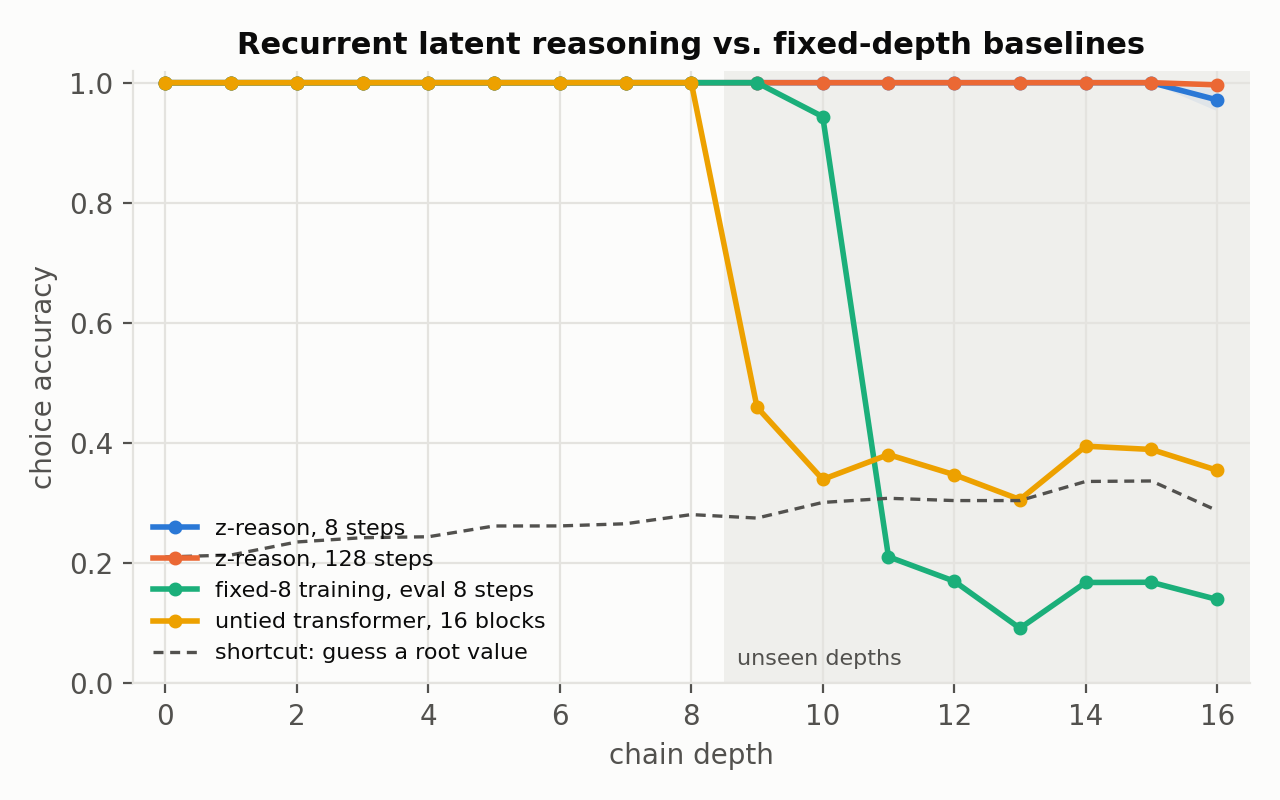
\includegraphics[width=0.62\textwidth]{figures/fig3_baselines.png}
\caption{Accuracy on \emph{choice} questions by depth, averaged over three seeds for \zr{}. All models solve the training range. Beyond depth 8, the untied transformer and the fixed-8 model evaluated at its training step count fall to the root guessing baseline, shown dashed, or below it, while \zr{} with 8 steps or more stays at or near 100\%.}
\label{fig:baselines}
\end{figure}

All three models solve the training range, as Table~\ref{tab:compare} shows, and they part ways as soon as they leave it, as Figure~\ref{fig:baselines} shows. The untied transformer has 3.7 times as many parameters but a fixed amount of computation, and it drops to 38\% at depths 9 to 12 and to 36\% at depths 13 to 16, close to the root guessing baseline. With random step training, \zr{} answers depths 9 to 16 with at least 99\% accuracy using 8 steps. Further out, with the step count fixed in advance at 32, it answers depths 16 to 20 with at least 98\% accuracy in all seeds, as reported in Table~\ref{tab:deep}. At depths 24 to 32, three to four times the training depth, two seeds remain between 93\% and 100\% while the third falls to between 63\% and 70\% at depths 28 to 32, and in this range accuracy is no longer monotone in the number of steps. Our claim is therefore robust extrapolation to twice the training depth and partial extrapolation beyond it.

The fixed-8 model shows that weight tying alone is not enough. At its training step count it behaves like the untied model beyond depth 10, and although more steps help it on average, its accuracy is not monotone in the number of steps. At depth 16 it reaches 100\% with 16 steps, 22\% with 24 and 94\% with 32, and over depths 1 to 16 adding steps can cost it as much as 78 points. For the models trained with random steps on the same depths, once accuracy has reached 99\% no larger step count up to 128 lowers it by more than 1.1 points in any seed. This is the overthinking phenomenon described for recurrent networks \cite{bansal2022endtoend} and for looped language models \cite{yang2026stars}, and training with random step counts is what makes the effect of \texttt{steps} predictable.

\subsection{Calibration}

\begin{table}[t]
\centering
\small
\caption{Accuracy and expected calibration error with 15 bins over all question types and depths 1 to 16, by number of test-time steps.}
\label{tab:calibration}
\begin{tabular}{lcccccc}
\toprule
test-time steps & 1 & 2 & 4 & 8 & 16 & 128 \\
\midrule
random steps, accuracy in \% & 66.8\,$\pm$\,0.2 & 82.1\,$\pm$\,0.7 & 95.4\,$\pm$\,0.3 & 100.0\,$\pm$\,0.0 & 100.0\,$\pm$\,0.0 & 100.0\,$\pm$\,0.0 \\
random steps, ECE & 0.041 & 0.019 & 0.014 & 0.000 & 0.000 & 0.000 \\
fixed 8, accuracy in \% & 32.6 & 58.5 & 75.5 & 92.3 & 96.4 & 96.3 \\
fixed 8, ECE & 0.358 & 0.306 & 0.187 & 0.060 & 0.028 & 0.028 \\
\bottomrule
\end{tabular}

\end{table}

\begin{figure}[t]
\centering
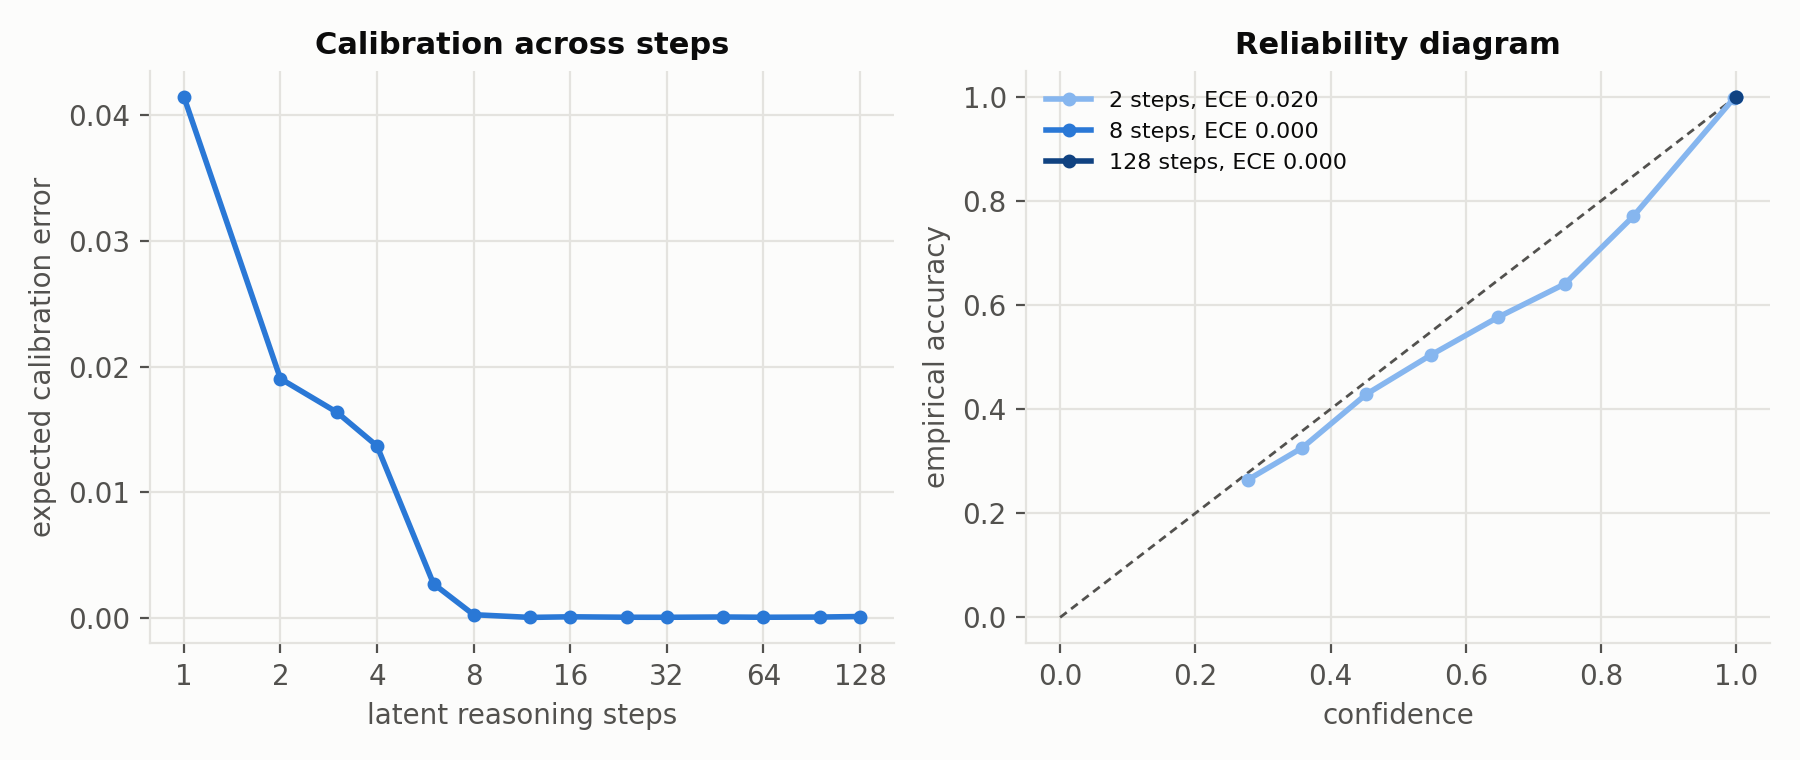
\includegraphics[width=0.85\textwidth]{figures/fig4_calibration.png}
\caption{Expected calibration error over all question types as a function of the number of test-time steps, on the left, and reliability diagram at 2, 8 and 128 steps, on the right.}
\label{fig:calibration}
\end{figure}

Downstream code may act on the answers by thresholding their probabilities, so calibration matters as much as accuracy. Table~\ref{tab:calibration} and Figure~\ref{fig:calibration} report the expected calibration error, or ECE. With few steps, when the model cannot yet resolve deep questions, its answers are uncertain but calibrated to within a few points. At two steps, over all question types and depths, the model is right about as often as it claims, with a reliability curve slightly below the diagonal. As steps increase, accuracy and calibration improve together, and the ECE stays below $10^{-3}$ from eight steps onward. The fixed-8 model, which was never trained to answer before step 8, is strongly overconfident with few steps and reaches an ECE of 0.36 with a single step.

This evidence is weaker than the numbers suggest. When the model is almost always right with a confidence close to 1, a vanishing ECE follows almost automatically. The informative regime is the one with few steps, or with inputs harder than the model can resolve, and there random step training produces useful calibrated probabilities from proper scoring rules alone. Testing calibration in a regime where the model stays uncertain after many steps would require a task that it cannot solve perfectly.

\subsection{Allocating steps automatically}

\begin{table}[t]
\centering
\small
\caption{Behavior of \texttt{steps="auto"} by depth, averaged over seeds, showing the mean number of steps used before the halting rule fires and the accuracy over all question types.}
\label{tab:auto}
\begin{tabular}{lccccccccc}
\toprule
depth & 1 & 2 & 4 & 6 & 8 & 10 & 12 & 14 & 16 \\
\midrule
mean steps used & 8.3 & 8.4 & 8.7 & 9.9 & 11.9 & 15.1 & 17.6 & 19.7 & 21.6 \\
accuracy in \% & 100.0 & 100.0 & 100.0 & 100.0 & 100.0 & 99.9 & 100.0 & 99.9 & 99.6 \\
\bottomrule
\end{tabular}

\end{table}

With \texttt{steps="auto"} the model stops once its answer distributions stop moving. Table~\ref{tab:auto} shows that the number of steps used then grows with depth, from about 8 at depth 1 to about 22 at depth 16, while accuracy stays between 99.6\% and 100\%. The rule is conservative, since it waits for convergence within $10^{-3}$ and therefore uses more steps than the minimum needed for 99\% accuracy shown in Figure~\ref{fig:needed}. A learned halting head could reduce this cost.

\section{What Did Not Work}
\label{sec:lessons}

\begin{table}[t]
\centering
\small
\caption{Design iterations that failed at this scale, each one isolated through controlled ablations.}
\label{tab:lessons}
\begin{tabular}{@{}p{4.6cm}p{4.5cm}p{4.9cm}@{}}
\toprule
Attempt & Symptom & Diagnosis and fix \\
\midrule
Character-level sequence, state encoded without access to the question, cosine similarity option head, GPT-style initialization $\mathcal{N}(0, 0.02^2)$ & loss stuck at $\ln 10$ even when looking up a single fact among three & bisection against a stock PyTorch transformer that learns the task showed that PyTorch default initialization, a dot product head and question-conditioned encoding were each required \\
Character-level reasoning with the fixes above & single lookups learned, but one-hop composition stuck at about 45\% \emph{choice} accuracy for more than 3{,}000 iterations under every variant tried, including other learning rates, batch sizes, noise levels and curricula & moving the recurrence from characters to fact vectors, after which one-hop composition was learned in about 2{,}000 iterations \\
Fact vectors read at a start token & start token vectors of different facts have cosine similarity of about 0.98 at initialization and nothing is learned & mean pooling over tokens \\
Concatenation adapter $W[z; e]$ \cite{geiping2025scaling} & input signal degraded by a randomly initialized projection at every step & additive injection $z + e$ \cite{bai2019deq, jolicoeur2025trm} \\
Random forest of variables & accuracy increased with depth & few roots made the root value guessable, fixed with independent chains, many roots and a reported baseline \\
Curriculum on a fixed schedule & training accuracy fell because difficulty grew faster than learning & adaptive curriculum \\
\bottomrule
\end{tabular}
\end{table}

A small model trained from scratch did not learn multi-hop lookup under most of the configurations we tried first. Table~\ref{tab:lessons} lists these failures and how each one was diagnosed. The most consequential concerned the unit of reasoning. Running the recurrence over characters, the most direct way to apply a latent reasoner to raw text, did not even learn to compose one lookup with another, while the same recurrence over fact vectors learned quickly. At this scale, reasoning over units larger than tokens made the difference between learning and not learning, which agrees with the motivation of concept-level modeling \cite{barrault2024lcm}. Another failure came from the task itself, whose first version contained a shortcut that produced what looked like strong extrapolation. We caught it only because accuracy rose with difficulty, and this is why every result in this paper is reported next to the root guessing baseline.

\section{Discussion and Limitations}
\label{sec:discussion}

In a setting where difficulty is controlled and shortcuts are measured, giving a typed decision model a user-chosen number of latent steps works as intended. More steps answer harder questions, the effect extends beyond the training distribution and the probabilities remain calibrated. The typed interface is untouched, because everything happens between the encoder and the read-out and the response schema is the same for any number of steps. For a user, the comparison with the step count of a diffusion sampler is apt. The parameter trades latency for quality, and random step training makes this trade close to monotone within the range where the model extrapolates reliably.

The scope of these results is narrow. They come from a single task, variable tracking over a clean and delimited input format in which the facts are given rather than extracted from prose and the vocabulary has 82 symbols. Carrying fact-level latent reasoning over to states written in natural language would require a pretrained text encoder, a way of segmenting free text into units and real decision data, and we have tested none of these. The model is small, with 4.1M parameters, and its questions have at most ten options, far from the 255 that Jev supports. The evidence on calibration is limited by saturated accuracy, and it relies on proper scoring rules rather than on an objective based on outcomes such as RLCD. The sublinear growth of the required steps is a behavioral finding, and our attention analysis does not identify the underlying algorithm. The \texttt{"auto"} mode is a convergence heuristic with a fixed tolerance. Extrapolation is robust only up to twice the training depth and varies across seeds at three to four times that depth, and the task cannot discriminate beyond depth 32 because of the limit on variable names. Finally, we compare with Jev only through its public interface, and nothing in this paper is a claim about its internals or its performance.

The most informative next step is a natural-language version of the task, with a pretrained sentence encoder in place of the character encoder. Tasks on which the model remains uncertain after many steps would allow a proper test of calibration, and a learned halting head and larger answer sets would bring the model closer to practical use.

\section{Conclusion}
\label{sec:conclusion}

System-One models trade the flexibility of text generation for fast, typed and calibrated decisions, and in doing so they give up test-time compute. On a controlled task we showed that this trade is not inevitable. A recurrent computation over fact-level latent vectors, exposed to the user as a number of steps and trained with random step counts, allows the same typed interface to spend more computation on harder questions. With it, a model with 4.1M parameters extrapolated reliably to twice its training depth and partially beyond, where a larger transformer of fixed depth did not, while its probabilities remained calibrated. These results establish the mechanism in a clean setting, and whether it carries over to decisions expressed in natural language is the natural next question.

\section*{Code and Data Availability}
The code, the task generator, the evaluation outputs and the scripts that produce every table and figure are available at \url{https://github.com/silvaan/z-reason}. The trained checkpoints will be made available at the same address.

\section*{Disclosure of AI Assistance}
The authors used Claude Opus 5.5 by Anthropic to assist with literature review, implementation and execution of the experiments, and drafting. The core idea, research question, direction, and all content decisions were the authors', who reviewed and verified all claims, results, and references, and take full responsibility for the final content.

\bibliographystyle{unsrtnat}
\bibliography{references}

\end{document}
